%%% The main file. It contains definitions of basic parameters and includes all other parts.

% Meta-data of your thesis (please edit)
\input metadata.tex

% Generate metadata in XMP format for use by the pdfx package
\input xmp.tex

%% Settings for single-side (simplex) printing
% Margins: left 40mm, right 25mm, top and bottom 25mm
% (but beware, LaTeX adds 1in implicitly)
\documentclass[12pt,a4paper]{report}
\setlength\textwidth{145mm}
\setlength\textheight{247mm}
\setlength\oddsidemargin{15mm}
\setlength\evensidemargin{15mm}
\setlength\topmargin{0mm}
\setlength\headsep{0mm}
\setlength\headheight{0mm}
% \openright makes the following text appear on a right-hand page
\let\openright=\clearpage

%% Settings for two-sided (duplex) printing
% \documentclass[12pt,a4paper,twoside,openright]{report}
% \setlength\textwidth{145mm}
% \setlength\textheight{247mm}
% \setlength\oddsidemargin{14.2mm}
% \setlength\evensidemargin{0mm}
% \setlength\topmargin{0mm}
% \setlength\headsep{0mm}
% \setlength\headheight{0mm}
% \let\openright=\cleardoublepage

%% If the thesis has no printed version, symmetric margins look better
% \documentclass[12pt,a4paper]{report}
% \setlength\textwidth{145mm}
% \setlength\textheight{247mm}
% \setlength\oddsidemargin{10mm}
% \setlength\evensidemargin{10mm}
% \setlength\topmargin{0mm}
% \setlength\headsep{0mm}
% \setlength\headheight{0mm}
% \let\openright=\clearpage

%% Generate PDF/A-2u
\usepackage[a-2u]{pdfx}

%% Prefer Latin Modern fonts
\usepackage{lmodern}
% If we are not using LuaTeX, we need to set up character encoding:
\usepackage{iftex}
\ifpdftex
\usepackage[utf8]{inputenc}
\usepackage[T1]{fontenc}
\usepackage{textcomp}
\fi

%% Further useful packages (included in most LaTeX distributions)
\usepackage{amsmath}        % extensions for typesetting of math
\usepackage{amssymb}        % extensions for typesetting of math
\usepackage{amsfonts}       % math fonts
\usepackage{amsthm}         % theorems, definitions, etc.
\usepackage{bm}             % boldface symbols (\bm)
\usepackage{booktabs}       % improved horizontal lines in tables
\usepackage{caption}        % custom captions of floating objects
\usepackage{dcolumn}        % improved alignment of table columns
\usepackage{floatrow}       % custom float environments
\usepackage{graphicx}       % embedding of pictures
\usepackage{indentfirst}    % indent the first paragraph of a chapter
\usepackage[nopatch=item]{microtype}   % micro-typographic refinement
\usepackage{paralist}       % improved enumerate and itemize
\usepackage[nottoc]{tocbibind} % makes sure that bibliography and the lists
			    % of figures/tables are included in the table
			    % of contents
\usepackage{xcolor}         % typesetting in color

% The hyperref package for clickable links in PDF and also for storing
% metadata to PDF (including the table of contents).
% Most settings are pre-set by the pdfx package.
\hypersetup{unicode}
\hypersetup{breaklinks=true}

% Packages for computer science theses
\usepackage{algpseudocode}  % part of algorithmicx package
\usepackage{algorithm}
\usepackage{fancyvrb}       % improved verbatim environment
\usepackage{listings}       % pretty-printer of source code

\usepackage{tikz}
\usepackage{tikz-uml}
\usetikzlibrary{positioning}

% You might want to use cleveref for references
% \usepackage{cleveref}

% Set up formatting of bibliography (references to literature)
% Details can be adjusted in macros.tex.
%
% BEWARE: Different fields of research and different university departments
% have their own customs regarding bibliography. Consult the bibliography
% format with your supervisor.
%
% The basic format according to the ISO 690 standard with numbered references
\usepackage[natbib,style=iso-numeric,sorting=none]{biblatex}
% ISO 690 with alphanumeric references (abbreviations of authors' names)
%\usepackage[natbib,style=iso-alphabetic]{biblatex}
% ISO 690 with references Author (year)
%\usepackage[natbib,style=iso-authoryear]{biblatex}
%
% Some fields of research prefer a simple format with numbered references
% (sorting=none tells that bibliography should be listed in citation order)
%\usepackage[natbib,style=numeric,sorting=none]{biblatex}
% Numbered references, but [1,2,3,4,5] is compressed to [1-5]
%\usepackage[natbib,style=numeric-comp,sorting=none]{biblatex}
% A simple format with alphanumeric references:
%\usepackage[natbib,style=alphabetic]{biblatex}

% Load the file with bibliography entries
\addbibresource{bibliography.bib}

% Our definitions of macros (see description inside)
\input macros.tex

%%% Title page and various mandatory informational pages
\begin{document}
%%% Title page of the thesis and other mandatory pages

%%% Inscriptions at the opening page of the hard cover

% We usually do not typeset the hard cover, but if you want to do it, change \iffalse to \iftrue
\iffalse

\pagestyle{empty}
\hypersetup{pageanchor=false}
\begin{center}

\large
Charles University

\medskip

Faculty of Mathematics and Physics

\vfill

{\huge\bf\ThesisTypeTitle}

\vfill

{\huge\bf\ThesisTitle\par}

\vfill
\vfill

\hbox to \hsize{\YearSubmitted\hfil \ThesisAuthor}

\end{center}

\newpage\openright
\setcounter{page}{1}

\fi

%%% Title page of the thesis

\pagestyle{empty}
\hypersetup{pageanchor=false}
\begin{center}

\centerline{\mbox{
\includegraphics[width=166mm]{img/logo-en.pdf}}}

\vspace{-8mm}
\vfill

{\bf\Large\ThesisTypeTitle}

\vfill

{\LARGE\ThesisAuthor}

\vspace{15mm}

{\LARGE\bfseries\ThesisTitle\par}

\vfill

\Department

\vfill

{
\centerline{\vbox{\halign{\hbox to 0.45\hsize{\hfil #}&\hskip 0.5em\parbox[t]{0.45\hsize}{\raggedright #}\cr
Supervisor of the \ThesisTypeName{} thesis:&\Supervisor \cr
\ifx\ThesisType\TypeRig\else
\noalign{\vspace{2mm}}
Study programme:&\StudyProgramme \cr
\fi
}}}}

\vfill

Prague \YearSubmitted

\end{center}

\newpage

%%% A page with a solemn declaration to the thesis

\openright
\hypersetup{pageanchor=true}
\vglue 0pt plus 1fill

\noindent
I declare that I carried out this \ThesisTypeName{} thesis on my own, and only with the cited
sources, literature and other professional sources.
I understand that my work relates to the rights and obligations under the Act No.~121/2000 Sb.,
the Copyright Act, as amended, in particular the fact that the Charles
University has the right to conclude a license agreement on the use of this
work as a school work pursuant to Section 60 subsection 1 of the Copyright~Act.

\vspace{10mm}

\hbox{\hbox to 0.5\hsize{%
In \hbox to 6em{\dotfill} date \hbox to 6em{\dotfill}
\hss}\hbox to 0.5\hsize{\dotfill\quad}}
\smallskip
\hbox{\hbox to 0.5\hsize{}\hbox to 0.5\hsize{\hfil Author's signature\hfil}}

\vspace{20mm}
\newpage

%%% Dedication

\openright

\noindent
\Dedication

\newpage

%%% Mandatory information page of the thesis

\openright
{\InfoPageFont

\vtop to 0.5\vsize{
\setlength\parindent{0mm}
\setlength\parskip{5mm}

Title:
\ThesisTitle

Author:
\ThesisAuthor

\DeptType:
\Department

Supervisor:
\Supervisor, \SupervisorsDepartment

Abstract:
\Abstract

Keywords:
{\def\sep{\unskip, }\ThesisKeywords}

\vfil
}

% In Czech study programmes, it is mandatory to include Czech meta-data:

\ifx\StudyLanguage\LangCS

\vtop to 0.49\vsize{
\setlength\parindent{0mm}
\setlength\parskip{5mm}

Název práce:
\ThesisTitleCS

Autor:
\ThesisAuthor

\DeptTypeCS:
\DepartmentCS

Vedoucí bakalářské práce:
\Supervisor, \SupervisorsDepartmentCS

Abstrakt:
\AbstractCS

Klíčová slova:
{\def\sep{\unskip, }\ThesisKeywordsCS}

\vfil
}

\fi

}

\newpage

%%% Further pages will be numbered, which LaTeX automatically enables at the next chapter start


\tableofcontents

\chapter*{Introduction}
\addcontentsline{toc}{chapter}{Introduction}

The integration of Multi-Material Unit (MMU) into Prusa 3D printer MK4 has promised a leap forward in printing capabilities, allowing for the use of multiple materials in a single print job. However, existing solutions, exemplified by the Prusa MMU3, present some practical challenges. This system is cumbersome, expensive, and prone to issues such as system crashes where diagnosing component failures becomes a difficult task. In light of these limitations, this bachelor thesis proposes a proof of concept for a more practical and efficient MMU solution.

The MMU3 enhances 3D printing capabilities by enabling the use of up to five different filaments in a single print job. It incorporates two motors, one for the filament selection and another for the filament pushing. The selector motor navigates a mechanism equipped with a filament sensor, to detect the presence of filament, ensuring the correct filament is aligned with the extruder’s intake path. The motor then engages, driving the sophisticated loading mechanism that feeds the filament into the extruder. This dual-motor setup allows for seamless switching between filaments, facilitating complex multi-material and multi-color printing.
In contrast, our design eliminates the selector motor. Each filament will have its own dedicated motor, and the selector's function will be handled by an innovative mechanical mechanism, streamlining the system and reducing complexity.

Through this thesis, we will explore the design, implementation, and testing of this MMU concept, with a focus on the firmware development process. By presenting a proof of concept for an improved MMU design, I aim to contribute to the advancement of additive manufacturing technology, paving the way for more efficient and user-friendly 3D printing systems.

The thesis is structured to provide a comprehensive understanding of the development and implementation of the MMU. The first chapter offers a technical overview that lays the groundwork by discussing 3D printing technologies. It details the components and processes essential for understanding the challenges in multi-material printing. The second chapter analyzes existing multi-material solutions, highlighting their limitations and setting the stage for the proposed improvements in the MMU. It defines the system requirements needed to enhance the 3D printing capabilities effectively. In the third chapter, the focus shifts to the system components of the MMU, detailing the electronic elements like microcontrollers, motor drivers, and sensors. This section explains the functionality of the Filament Hub, which is central to the proposed improvements. The fourth chapter describes the development environment and tools used in the project, emphasizing the build systems, testing frameworks, and deployment strategies that support the firmware development. The firmware architecture is explored in the fifth chapter, where the firmware design and modular approach are discussed to ensure scalability and integration of future enhancements. Implementation details are provided in the sixth chapter, covering the specifics of protocol management, motor control, sensor integration, and data transmission, crucial for the interaction between the MMU and the printer. The seventh chapter evaluates the performance of the MMU, assessing aspects such as usability, reliability, and efficiency based on testing and user feedback. This evaluation helps identify areas for potential improvement. The thesis concludes by summarizing the significant contributions made towards advancing 3D printing technology and outlining future directions for the research and development of the MMU system. Each chapter builds on the previous ones, progressively detailing the development and refinement of a more efficient MMU for 3D printers.








\chapter{Technical overview}

The developement of the MMU for 3D printer requires an understanding of several key concepts and technologies. This chapter aims to provide the neccessary background and context to better understand the MMU implementation discussed in later chapters. Even for those already familiar with the subject, a brief refresher might be helpful.

\section{Understanding 3D print technology}

Let us start with what 3D print is and what it does.
3D printing technology, also known as additive manufacturing, enables the creation of three-dimensional objects by layering materials based on digital models. This process has unlocked new avenues for innovation, allowing designers, engineers, and hobbyists to bring their ideas to life in a tangible form. In this chapter, we will delve into the fundamentals of 3D printing technology, with a focus on the popular Fused Deposition Modeling (FDM) method utilized in Prusa 3D printers. By understanding the underlying principles of FDM technology.

\section{Fused Deposition Modeling}

Fused Deposition Modeling (FDM) \cite{fdm} technology has revolutionized manufacturing and prototyping by offering a cost-effective and accessible method for creating three-dimensional objects. By understanding the principles of FDM printing, users can harness the full potential of this technology to bring their ideas to life with precision and efficiency.

Advantages of FDM Technology are cost-effectiveness: FDM printers are relatively affordable compared to other 3D printing technologies, making them accessible to a wide range of users, FDM printers are user-friendly and require minimal setup, making them ideal for beginners and experienced users alike, FDM enables rapid iteration and prototyping, allowing designers to quickly test and refine their ideas.

\subsection{Printing process}

\subsubsection{Slicing for FDM}
The process begins with the creation or acquisition of a 3D model in a computer-aided design (CAD) software. The model is then exported as a STL \cite{stl} file, which contains the geometric information needed for printing.
Slicing software, such as PrusaSlicer \cite{slicer}, processes the STL file and generates a G-code \cite{gcode} file containing detailed instructions for the printer's movements, such as the path the print head should follow, the amount of filament to extrude, and the temperature settings

\subsubsection{Printing}
Once the slicing is complete, the sliced file is transferred to the 3D printer. The printer heats the thermoplastic filament to its melting point and extrudes it through the nozzle onto the build platform. The nozzle moves in accordance with the instructions from the sliced file, depositing each layer of material until the object is fully formed. After printing, the object may require post-processing steps such as removing support structures.


\section{Extruder}

Understanding the extruder component is crucial for a MMU project because it directly influences material handling, filament control, compatibility, software integration, and troubleshooting. Extruder, see Figure~\ref{fig:extruder}, is responsible for pushing filament through the hotend, melting it, and depositing it onto the print bed. In an MMU setup, where multiple filaments are used, knowing the extruder helps in handling different materials effectively. It ensures proper control over filament flow, enabling smooth transitions between materials. Different extruders have varying capabilities and limitations, making it essential to select the right one for the MMU project \cite{3d-print-basics}. Understanding the extruder is particularly vital when implementing a new MMU system, as it lays the groundwork for optimizing the mechanical and electronic coordination required for managing multiple materials. This knowledge aids in integrating it with software systems for coordinated filament loading and switching. Moreover, troubleshooting issues like under-extrusion or jamming requires knowledge of the extruder's operation to diagnose and resolve problems efficiently. Overall, a comprehensive understanding of the extruder is essential for a successful implementation and operation of the MMU project, ensuring high-quality prints with multiple materials.

\begin{figure}[ht]
    \centering
    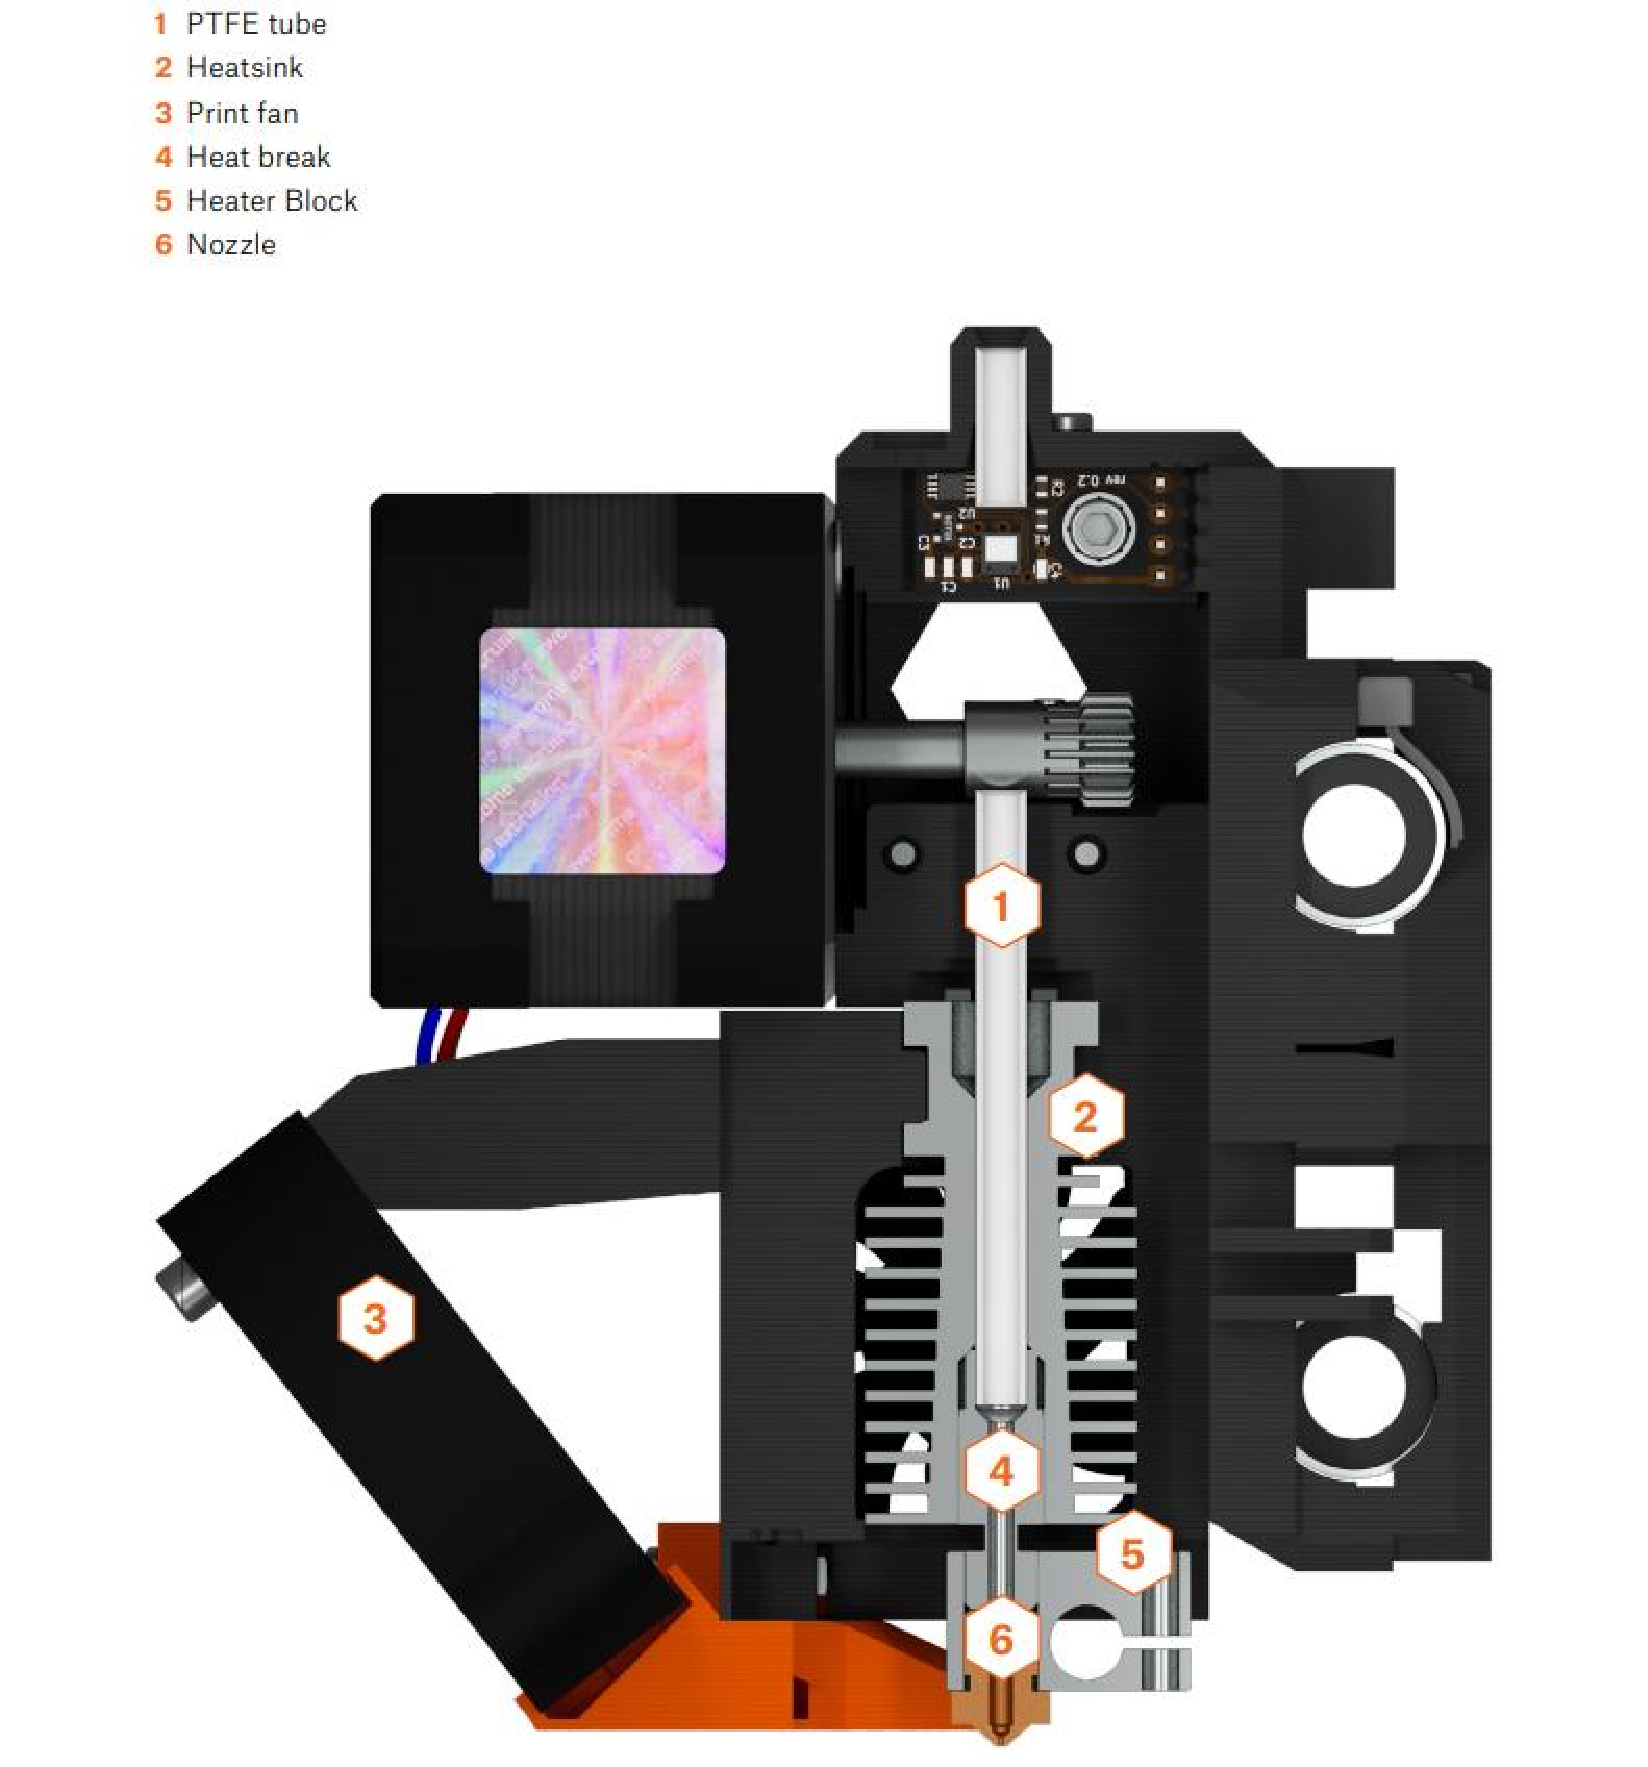
\includegraphics[width=0.8\linewidth]{img/extruder_prusa}
    \caption{Detail of the extruder}
    \label{fig:extruder} 
\end{figure}

\subsection{Heatsink}

The heatsink is part of the extruder that dissipates heat away from the hotend, preventing the filament from melting too early as it travels down the extruder assembly. It is usually attached directly above the heat break and features fins or ridges to increase the surface area, improving its ability to cool by air flow provided by the print fan.

\subsection{Print fan}

The print fan is designed to blow air directly onto the printed material as it exits the nozzle, helping in cooling the material immediately after deposition. This rapid cooling is essential for preventing warping and ensuring good adhesion between layers.

\subsection{Heat break}

The heat break is a narrow and often thermally conductive component that connects the heatsink and the heater block. Its primary function is to restrict the flow of heat upwards, ensuring the filament remains solid until it reaches the heater block, which is critical in maintaining consistent extrusion and preventing jams.

\subsection{Heater block}

The heater block is a metal block that surrounds the heat break and houses the heating element and temperature sensor. Its primary role is to evenly distribute heat to melt the filament precisely before it is pushed through the nozzle. The block maintains a consistent temperature.

\subsection{Nozzle}

The nozzle is the component at the very tip of the extruder that directs the molten filament onto the print bed. Nozzles come in various diameters which influence the resolution and speed of printing; smaller nozzles produce finer details, while larger nozzles allow for faster print speeds

\subsection{Polytetrafluoroethylene tube}

The Polytetrafluoroethylene (PTFE) tube \cite{ptfe} guides the filament from the filament spool to the hotend. It minimizes friction due to its low coefficient of friction, allowing for easier and more reliable filament feeding.

\section{Physics backround}

In this section, we will focus on the fundamental principles of DC motors and Hall effect, which are two pivotal concepts MMU hardware system is based on. 

\subsection{Direct current motor principle}

Direct current (DC) motor is a type of electrical machine that converts electrical energy into mechanical energy through the interaction of magnetic fields. It works on the principle of the Lorentz force, which states that a current-carrying conductor placed within a magnetic field experiences a force. This fundamental principle is harnessed in a DC motor to produce rotational motion.

When a DC motor is powered, an electric current flows through the armature coil. The magnetic field produced by the stator interacts with the magnetic field generated by the electrified armature. According to the left-hand rule of Fleming, which predicts the direction of the force acting on a current-carrying conductor in a magnetic field, this interaction creates a force perpendicular to both the direction of the current and the magnetic field. This force generates torque at the armature, causing it to spin.
A
DC motors are valued for their simple design and easy control, high reliability and torque at low speeds, and cost-effectiveness across a wide range of applications \cite{dc-motor}.

\subsection{Hall effect}

The Hall effect occurs when an electric current flows through a conductor with a magnetic field applied perpendicular to the current. This interaction generates a voltage across the conductor, which is perpendicular to both the current and the magnetic field. The Hall effect is useful for measuring magnetic field strength and determining the type of charge carried in a material. It is also employed in various devices like Hall effect sensors, which are used to measure magnetic fields, speed, and proximity in many applications \cite{hall-effect}.

\chapter{Analysis}

To evaluate the feasibility of the proposed MMU, it is essential to analyze existing alternatives. This chapter will provide a thorough examination of alternative solutions, underscoring their drawbacks and limitations. Additionally, we will explore the necessary requirements for the implementation of MMU system.

\section{Analysis of alternatives}

\subsection{Multiple extruder heads}

In this configuration, each extruder is equipped with its own nozzle, and is specifically dedicated to a distinct type of filament. Multiple extruders are mounted on the gantry of the printer. These may be positioned side by side or designed to activate sequentially. The printer's control system switches between these extruders based on the material requirements of different sections of the print. This setup demands meticulous calibration to ensure that each nozzle is precisely aligned at the same height to prevent any interaction with the part being printed, which could result in damage to both the print and the printer. This strategy is exemplified by the printer Prusa XL \cite{prusa-xl}.

\subsection{Single extruder head with one motor for filament pushing}

The central element of this system is a selector motor, tasked with choosing the active filament. The motor maneuvers a mechanical selector to align with the intended filament’s feed path, thus enabling seamless switching between different filaments during the printing process. After selection, a single motor for filament pushing engages to pull the chosen filament toward the printer’s extruder. The precision of the motor for filament pushing is essential to ensure consistent filament feed and prevent slippage, which is vital for maintaining print quality. The system also incorporates an idler mechanism that works in tandem with the motor for filament pushing to maintain appropriate tension on the filament, preventing tangling and ensuring smooth filament delivery. However, the reliance on a single selector and motor for filament pushing can increase mechanical complexity and potential failure points. This arrangement is utilized by the Prusa MMU3 for MK4.

\subsection{Single extruder head with multiple motors for filament pushing}

Each filament spool in this system is equipped with a dedicated motor for filament pushing. This motor plays an important role in ensuring that the filament is fed smoothly and consistently into the printer. Central to the system is the Filament Hub, which works as the control center that manages the filament's journey from the spool to the printer. This hub is outfitted with various sensors that continuously monitor the filament's presence and movement. These sensors are crucial for detecting any irregularities such as filament run-outs or jams. If a run-out or jam is detected, the system can automatically pause the printing operation, alerting the user to the issue and preventing damage or wastage. Given the fact, that the implementation of the first approach is nearly impossible for the MK4, and the second approach is already in use, this thesis will focus on exploring the third variant.

\section{System requirements}

In developing firmware for systems where mechanical solutions have already been decided, it is time to thoroughly inspect the system requirements. 

The primary function of the MMU is to manage multiple input filaments to select and feed the appropriate filament to the printer’s bondtech gears for trouble-free printing operations.

Drawing inspiration from the Prusa MMU3 \cite{prusa-mmu3}, which operates under the master-slave principle \cite{master-slave}, our implementation will similarly designate the printer as the master and the MMU as the slave. This setup utilizes a specific MMU port on the printer to relay commands, ensuring that the MMU is capable of proper communication. While the communication protocol of the Prusa MMU3 provides a starting point, it will require adjustments to tailor it to our system's specific needs, enhancing its efficiency and reliability in our targeted applications.

\subsection{MMU functionality}

The MMU should manage the following functions:
\begin{itemize}
    \item \textbf{Load filament}: This function should be responsible for positioning the filament in readiness for printing. It parks the filament before the Filament Hub, preparing it for engagement with the rest of the machine's feeding system. This step ensures that the filament is properly aligned and ready for a seamless feed into the printer.
    \item \textbf{Eject filament}: This function fully unloads the filament from the MMU and the associated bowden tube after printing is complete. This step is crucial for clearing the entire path, ensuring that no filament remnants obstruct or interfere with subsequent filament loads, thereby preventing any potential jams or material mixing within the printer’s mechanism.
    \item \textbf{Load filament to nozzle}: This function aids the extruder by pushing the filament towards and into the nozzle. It ensures that the filament is fed consistently and reaches the nozzle without any interruptions, which is vital for accurate and quality printing.
    \item \textbf{Unload filament from nozzle}: This function retracts the filament from the nozzle and parks it before the Filament Hub. It should be designed to disengage the filament from the printing area, preparing it for ejection or for being securely stored away from the primary mechanical pathways. This action helps to achieve a smooth transition between different filaments without cleaning or additional maintenance interventions.
    \item \textbf{Tool change}: This function is the most complex one. It essentially consists of the two previously mentioned commands: Load filament to nozzle and Unload filament from nozzle.
\end{itemize}

While the printer is idle, all these operations can be manually initiated by the user from a stand-alone mode through the MMU menu. This capability does not require any special implementation, as the MMU operates as a slave device and merely carries out the commands from the printer. Furthermore, since the menu system is already developed for the Prusa MMU3, this functionality should be readily available without additional cost.

\subsection{Communication with printer}

Initially, the intention was to employ CAN bus \cite{can}, a modern communication medium extensively utilized in automotive applications. This solution, while complex, was considered potentially beneficial. Unfortunately, the MK4 does not have CAN bus connectivity available on its board. Consequently, the alternatives narrowed down to either RS232 or RS485 \cite{uart}.

For a time, we contemplated using the Modbus protocol \cite{modbus} over RS485, since this protocol is already integrated into the MK4 printer for internal communications. However, this option was quickly dismissed due to prior experiences. Modbus, while robust and well-established in industrial automation, tends to involve substantial overhead both in terms of the byte count necessary for data transmission and its framing structure. Given its age and design focus, Modbus might not support some features offered by more contemporary protocols.

The final decision was to continue using the text protocol over RS232, as it is currently employed in the existing Prusa MMU3 setup via UART. There is no compelling reason to deviate significantly from this existing protocol, as it meets our needs well. Adjustments will be minimal since not all aspects of the current implementation are required. Additionally, the printer is already configured to UART at a baud rate of 115200, making this a practical choice.

\chapter{System components}

This chapter provides a comprehensive examination of the electronic components and systems integrated into the MMU system. It begins with a key decision made independently—the selection of the microcontroller. Further, this the chapter introduces choices made by the electronics team, detailing the roles and specifications of other components such as DC motors, motor drivers, and Hall effect sensors. These components ensure precise operation and control within the MMU. Through technical descriptions and schematic overviews, the chapter not only highlights the functionalities of these components but also illustrates their integration and interaction within the MMU system.

\section{Microcontroller}

\subsection{Microcontroller analysis}

When considering microcontrollers for MMU project, the choices from Texas Instruments, STMicroelectronics, and AVR each come with their distinct advantages and typical usage scenarios.

Texas Instruments microcontrollers are known for their low power consumption, which makes them suitable for battery-operated devices like portable health monitors and smart sensors. They feature advanced power management capabilities that help extend their operational lifetime in energy-sensitive applications. Additionally, Texas Instruments provides a wide array of microcontroller options that support various wireless communication protocols.

STMicroelectronics, particularly the STM32 series used in the MK4 printer, is preferred for its high performance and broad range of features. These microcontrollers provide powerful processing capabilities and flexible connectivity options, including USB, Ethernet, and Bluetooth. They are ideal for complex applications such as multimedia processing and IoT devices that handle various data types. However, these microcontrollers generally have higher power consumption, which may not be suitable for the most power-sensitive projects.

AVR microcontrollers, currently used in the MMU, are noted for their simplicity and ease of use. They are particularly well-suited for rapid prototyping and small-scale projects thanks to easy programming and integration. While their performance adequately meets the needs of many applications, such as simple robotics and home automation systems, they may lack the necessary processing power for more demanding tasks. Compared to Texas Instruments and STM, AVR microcontrollers may offer fewer resources and less advanced peripherals.

In summary, the selected microcontroller for this project is the MSPM0G3507 from Texas Instrumentso \cite{mspm0g3507}. The MSPM0G3507 provides performance comparable to the STM32 but at a lower cost than AVR, making it a compelling choice \cite{avr-price}.

\subsection{MSPM0G3507}

The MSPM0G3507 microcontroller is a highly integrated, ultra-low-power device designed for a range of applications from motor control to factory automation. Based on the Arm Cortex-M0+ core \cite{arm-cortex} operating at up to 80 MHz, it features robust digital and analog capabilities. This includes up to 128KB of flash memory with error correction and up to 32KB of SRAM with hardware parity. Its analog capabilities are substantial, with multiple high-speed ADCs and DACs, comparators, and zero-drift amplifiers, which make it suitable for precise measurement and control tasks.

The microcontroller also supports a range of communication protocols including multiple UART interfaces, I2C, SPI, and CAN-FD, making it versatile for different communication needs. It is built to operate in a wide range of environmental conditions, supporting temperatures from -40°C to 125°C and a voltage range from 1.62V to 3.6V.

For power management, it offers several low-power modes that significantly reduce energy consumption when idle or in standby, which is essential for battery-operated devices. The device includes advanced security features such as AES encryption and a true random number generator, ensuring data integrity and security in sensitive applications \cite{mspm0-manual}.

\section{Direct current motor}

In MMU, DC motors are used to manage the filament selection process. Each filament type is loaded into a separate channel within the MMU, and the DC motor is responsible for driving the selected filament towards the extruder. This system allows for switching between different filaments during a single print job.

In the Figure~\ref{fig:dc_motor_ic}, on the left there is an X-ray image of an integrated circuit, showcasing the internal components of a motor. The X-ray gives us a clear view of the layout and structure within the device. On the right side, there is a neatly organized schematic diagram. This serves as a visual guide to the motor's circuitry, detailing the connections and components. Together, these two elements offer a comprehensive overview of the motor's design.

\begin{figure}[H]
    \centering
    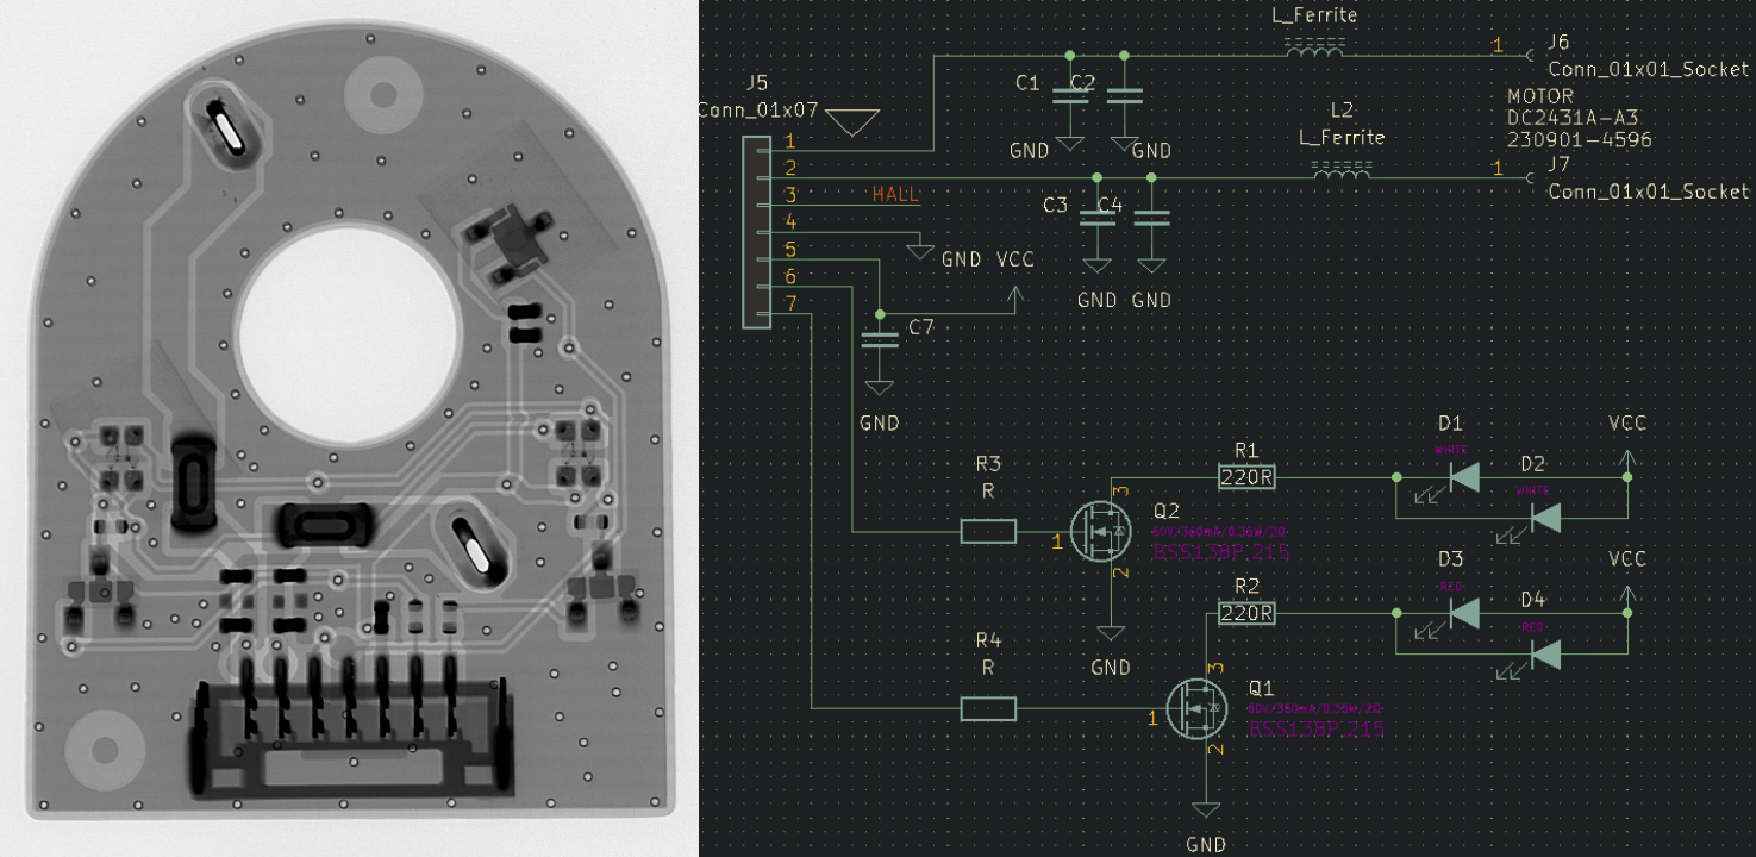
\includegraphics[width=0.8\linewidth]{img/dc_motor}
    \caption{DC motor}
    \label{fig:dc_motor_ic} 
\end{figure}

\section{Direct current motor driver}

The Pololu TB6612FNG Dual Motor Driver Carrier \cite{motor-driver} is a compact module that allows for control of two bidirectional DC motors or one bipolar stepper motor. It utilizes Toshiba's TB6612FNG motor driver integrated circuit. The board supports a motor voltage range of 4.5V to 13.5V and can deliver up to 3A per channel in peak output with a continuous current of 1A per channel, which can be increased to 2A if channels are paralleled. The logic voltage can be between 2.7V and 5.5V. It includes built-in thermal shutdown, filtering capacitors on both supply lines, and reverse-power protection on the motor supply.

\section{Hall effect sensor}

A Hall effect sensor is a type of magnetic sensor, which when exposed to a magnetic field perpendicular to the current's flow in a conductor, a voltage—known as Hall voltage—is generated across the conductor. This voltage is perpendicular to both the current and the magnetic field, allowing the sensor to detect the strength and changes in the magnetic field.

In this project, the MT9105 variant \cite{hall-effect-sensor} from the MT910X series of linear Hall effect is utilized. The MT9105 operates within a 3.0V to 5.5V voltage range and outputs a voltage at half of the supply voltage when no magnetic field is present. The sensor's output varies linearly with the magnetic flux density, offering different sensitivity settings to maximize output voltage swing based on the required sensing range. It also responds distinctly to the north and south poles of a magnet.

\section{Filament Hub}

The role of the Filament Hub is to keep the PTFE tubes, corresponding to each slot of the MMU, organized and held together, thus ensuring smooth feeding of the filament to the extruder.

On the circuit board, in Figure~\ref{fig:hub_ic}, three MT9105 Hall sensors are installed, each serving a different function. The filament sensor connector includes duplicate power supply pins and three analog outputs corresponding to these sensors. The first output is connected to a Hall sensor that detects the presence of filament in the extruder. The second output is linked to another Hall sensor that monitors the cutting blade's interaction with the filament; however, there is currently no implemented solution for cutting, making this sensor non-functional for its intended purpose. The third output measures the tension of the filament in the Bowden tube.

\begin{figure}[H]
    \centering
    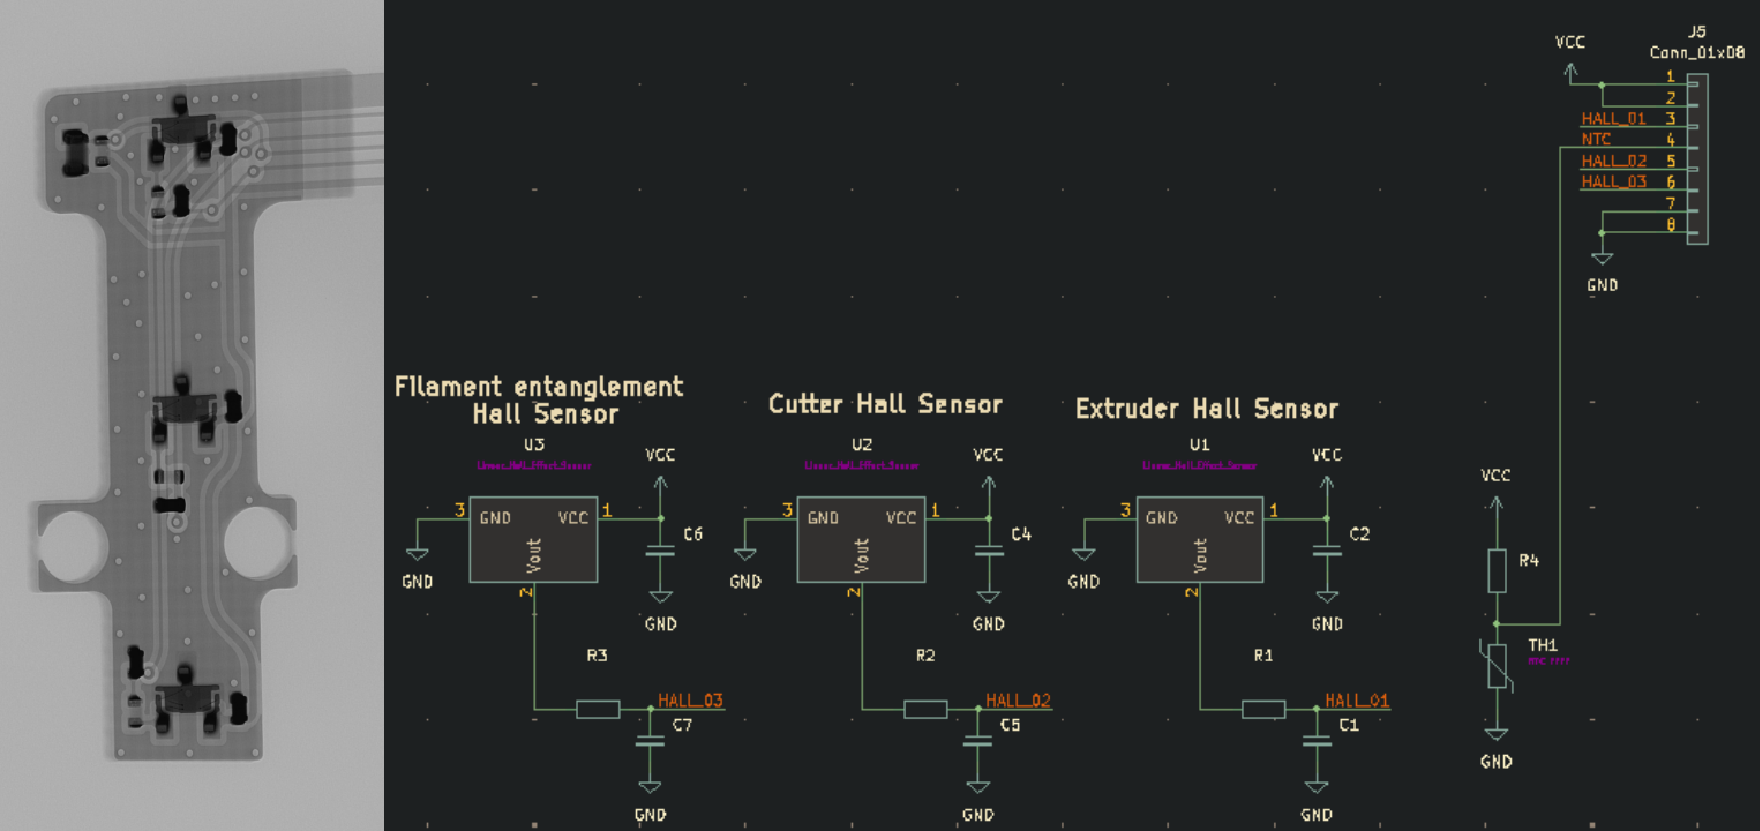
\includegraphics[width=0.8\linewidth]{img/filament_hub}
    \caption{Filament Hub}
    \label{fig:hub_ic} 
\end{figure}

\section{Filament sensor in feeding system}

The filament sensor in MMU feeding system acts as a guard and ensures smooth passage of filament from the spool to the printer's extruder. The sensor's main function is to detect the presence of filament and alerts the system to any shortage or breakage that could interrupt printing. This early detection allows the printer to pause and offers the user an option to rectify the issue without compromising the print job.

By monitoring the movement and flow of the filament, the sensor helps the printer adjust the pull from the spool in real-time, reducing the risk of knots or obstructions that could lead to print failure. Furthermore, the filament sensor facilitates automated loading and unloading of filament.

The Figure~\ref{fig:fsensor_ic} displays an X-ray image of an integrated circuit of filament sensor in the feeding system.

\begin{figure}[H]
    \centering
    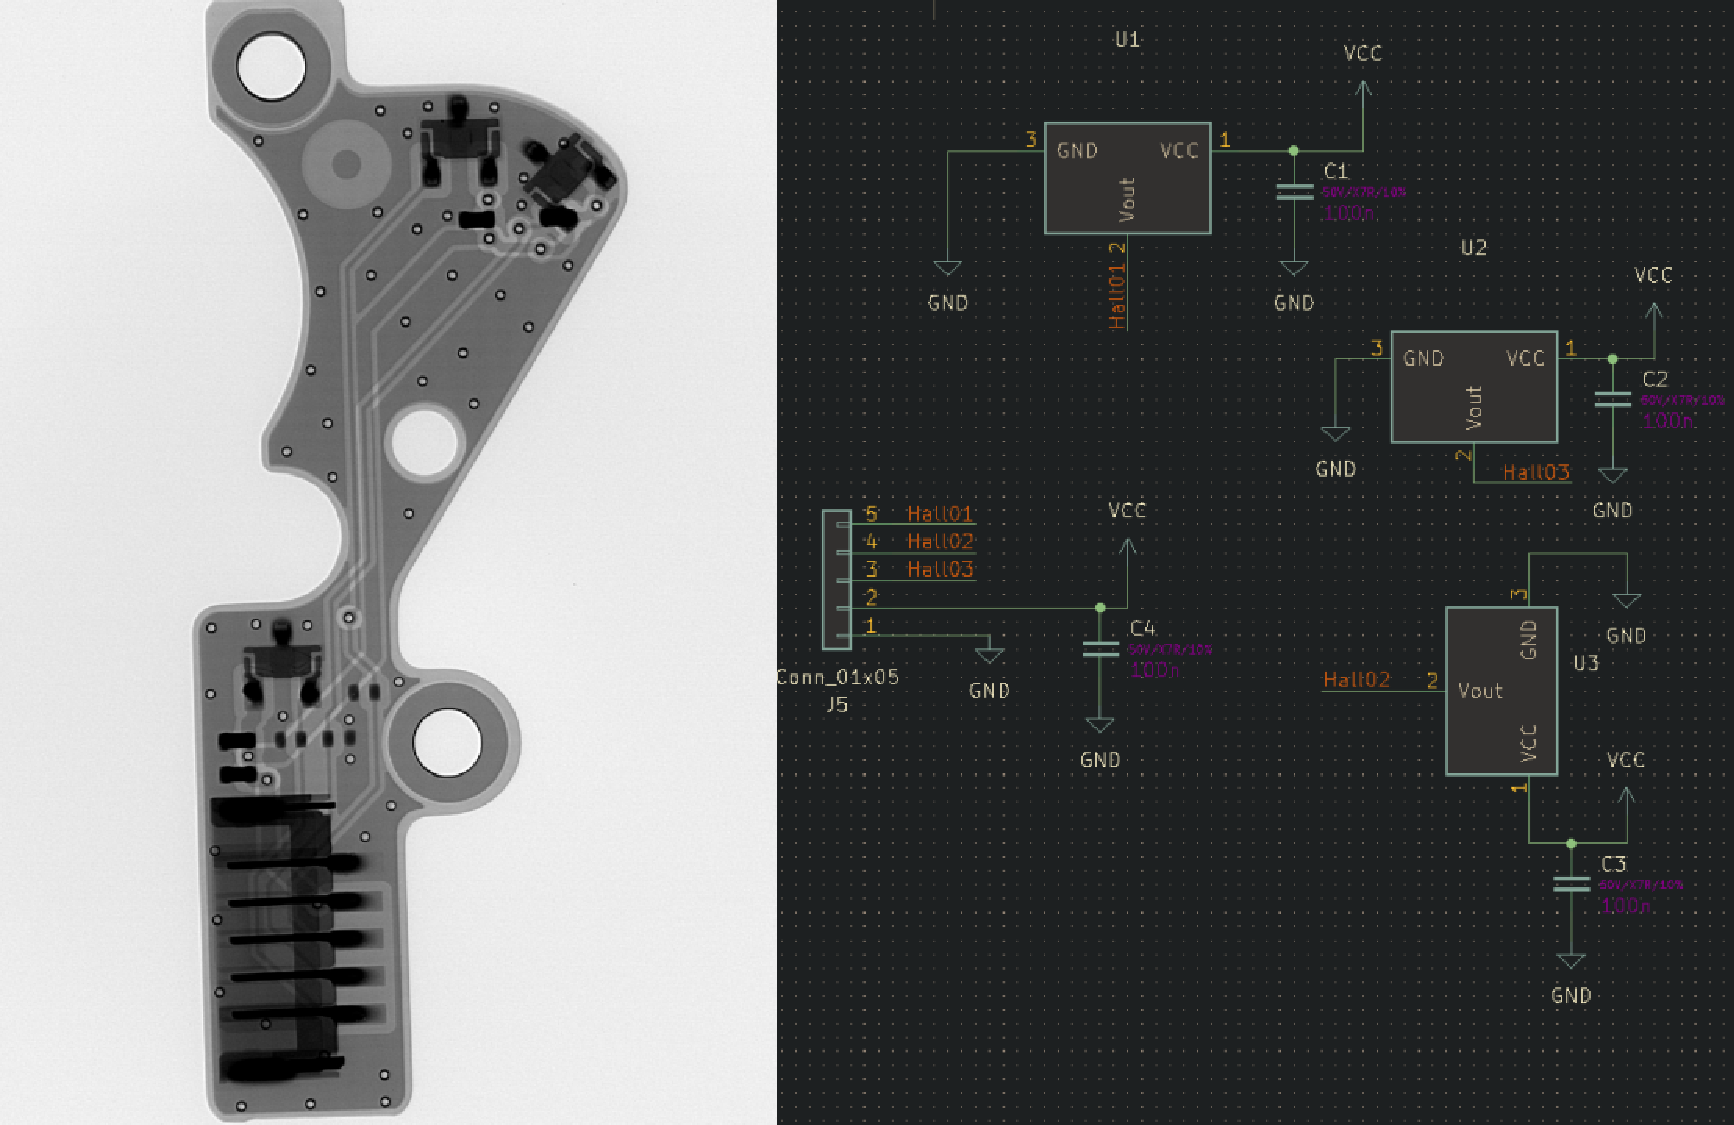
\includegraphics[width=0.8\linewidth]{img/filament_sensor}
    \caption{Filament sensor}
    \label{fig:fsensor_ic} 
\end{figure}

\chapter{Development environment and developement tools}

\section{Build system}

Texas Instruments offers specialized build tools tailored for controller hardware configuration, known as SysConfig \cite{sysconfig}. SysConfig is instrumental in streamlining the configuration process of the hardware, allowing developers to adjust hardware settings and parameters through a user-friendly interface. This tool generates configuration files that are integral in defining how the hardware operates, optimizing hardware utilization for specific applications.

Alongside SysConfig, Texas Instruments also provides tools for building the software system. These tools are capable of automatically generating makefiles, which are essential for managing the build process of the software. Makefiles \cite{make} created by these tools ensure that the compilation process is efficient and manages dependencies and compilation rules in a way that enhances the build execution.

Furthermore, for the development and maintenance of high-quality software, unit testing is crucial. Unit tests are built using CMake \cite{cmake}, a robust open-source system that facilitates the process of compiling, linking, and testing the application. CMake supports cross-platform builds and is favored for its ability to generate makefiles and project files that can be used in various integrated development environments. This feature is particularly useful for testing environments where consistency across different development platforms is required.

Incorporating these tools into the development process ensures a seamless transition from hardware configuration to software deployment, enhancing the efficiency and reliability of the development process. Each component—from SysConfig for hardware configuration, automated makefile generation for software builds, to CMake for unit testing—plays a pivotal role in the lifecycle of firmware development, ensuring that both hardware and software are optimally configured and tested before deployment.

\section{Testing framework}

Firmware testing involves verification process that establishes whether the code performs as expected under real-world operational conditions. For this purpose, Google Test \cite{google-test} has been selected as the testing framework thanks to its integration with Google Mock \cite{google-mock}, which facilitates comprehensive testing scenarios including mocking capabilities. While Catch2 \cite{catch2} is also considered, it has not been chosen because it lacks built-in support for mocks. To enhance the testing process, data is collected directly from the printer during operation, which is then utilized as an input for unit tests to ensure that tests are grounded in actual performance metrics.

\section{Deployment}

The Docker container \cite{docker} is set up for the project; however, it is not recommended to develop code directly within it. The project’s makefile is generated automatically by Texas Instruments developement tools \cite{ccs}, meaning the Docker environment is better suited as a deployment tool rather than a development environment. This setup helps ensure that the development process remains consistent and manageable across different systems, while Docker primarily handles the integration and deployment phases.


\chapter{System architecture}

In this chapter, we will focus on decisions from the perspective of the system's architecture.

\section{Firmware architecture}

The firmware of the MMU is strategically designed around a state machine architecture, tailored to efficiently manage a wide array of simple states required by its operations. This system is particularly effective due to the MMU's role as a slave device that exclusively receives and executes commands from a printer.

One key design decision is the omission of a real-time operating system to keep the system as resource-efficient as possible. Consequently, all sensor and motor controls are either interrupt-driven or blocking, which is not ideal but it has been chosen to simplify the system.

Another important strategy in the MMU firmware design is the avoidance of dynamic memory allocation. Dynamic allocations can lead to memory fragmentation, which, in an embedded system like the MMU, can cause severe issues such as memory leaks and system crashes. Instead, the firmware uses references to already created objects and resets the state of these objects as necessary. This approach minimizes the need for new memory allocations during runtime, enhancing the system’s stability and performance by maintaining a predictable memory footprint.

\subsection{Architectural overview}

At the core of the system is the \texttt{App} class, which facilitates access to communication mediums and handles messages received through these mediums, parsed by the \texttt{Protocol} class.

Commands are categorized into two types: specific commands that execute respective actions and composite commands that are composed of multiple specific commands. This structure allows for dynamic and flexible command processing, tailored to the complex requirements of the system.
\texttt{CommandBase} serves as the abstract base for all commands, providing basic structure and methods. Derived from this base class are \texttt{ConcreteCommandBase} and other specific command classes like \texttt{LoadFilamentCommand}.

Moreover, \texttt{ConcreteCommandBase} introduces more specialized members. Class \texttt{FeedingSystem} handles the coordination and operational logic of motor-driven feeding mechanisms, utilizing sensors to monitor and control the state of the filament. It serves as a high-level abstraction for the feeding mechanism, enabling actions like monitoring filament presence, adjusting motor operations, and responding to operational anomalies. Additionally, \texttt{HubFilamentSensor} the and \texttt{Registers} components abstract the interactions with hardware sensors and system registers, respectively. These abstractions help manage the complexity of direct hardware manipulation and promote a modular approach to system design.

Main classes and their relationships are illustrated in Figure~\ref{fig:uml_diagram}, showing their inheritance and methods.

\begin{figure}[ht]
    \centering
    \scalebox{1}{
        \begin{tikzpicture}[every node/.style={font=\scriptsize}, node distance=1cm]
    % Base Command class
    \begin{scope}[scale=0.8, transform shape]
    \umlclass[x=-2, y=0]{App}{
        -- CommandBase* currentCommand\\
	-- Protocol protocol \\
	-- Communication communication
    }{
        + Step (\ldots) \\
        + PlanCommand (\ldots) \\
        + CheckMessages (\ldots) \\
        + \ldots
    }
    \end{scope}

    \begin{scope}[scale=0.8, transform shape]
    \umlclass[x=3, y=-5]{CommandBase}{
        -- ProgressCode state \\
        -- ErrorCode error \\
    }{
	+ Step() \\
	+ Reset() \\
        + virtual StepInner() \\
        + virtual ResetInner()
    }
    \end{scope}
    
    \begin{scope}[scale=0.8, transform shape]
    \umlclass[x=-5, y=-5]{ConcreteCommandBase}{
        -- FeedingSystem (\&feedingSystems)[ ] \\
        -- HubFilamentSensor\& sensor \\
        -- Registers\& registers
    }{
        + virtual StepInner() \\
        + virtual Reset() \\
	+ Unstuck()
    }
    \end{scope}

    \begin{scope}[scale=0.8, transform shape]
    \umlclass[x=-5, y=-13]{UnloadFromNozzleCommand}{
    }{
        + StepInner() override \\
        + Reset() override
    }
    \end{scope}

    \begin{scope}[scale=0.8, transform shape]
    \umlclass[x=-8, y=-10]{LoadFilamentCommand}{
    }{
        + StepInner() override \\
        + Reset() override
    }
    \end{scope}

    \begin{scope}[scale=0.8, transform shape]
    \umlclass[x=-1, y=-10]{LoadToNozzleCommand}{
    }{
        + StepInner() override \\
        + Reset() override
    }
    \end{scope}

    \begin{scope}[scale=0.8, transform shape]
    \umlclass[x=-4, y=-16]{EjectFilamentCommand}{
    }{
        + StepInner() override \\
        + Reset() override
    }
    \end{scope}

    \begin{scope}[scale=0.8, transform shape]
    \umlclass[x=3, y=-15]{ToolChangeCommand}{
	-- LoadToNozzleCommand\& \\
	-- UnloadFromNozzleCommand\& 
    }{
        + StepInner() override \\
        + Reset() override
    }
    \end{scope}

    % Associations
    \umlaggreg{App}{CommandBase}
    \umlinherit{ConcreteCommandBase}{CommandBase}
    \umlinherit{UnloadFromNozzleCommand}{ConcreteCommandBase}
    \umlinherit{LoadFilamentCommand}{ConcreteCommandBase}
    \umlinherit{LoadToNozzleCommand}{ConcreteCommandBase}
    \umlinherit{EjectFilamentCommand}{ConcreteCommandBase}
    \umlinherit{ToolChangeCommand}{CommandBase}
\end{tikzpicture}

    }
    \vspace{15pt}
    \caption{UML diagram of the system architecture.}
    \label{fig:uml_diagram}
\end{figure}

\subsection{Portability}

The MMU is built on top of the Driver Library \cite{driver-lib} made by Texas Instruments, which interfaces directly with hardware registers. This library does not automate all functionalities; manual configuration through are necessary for all hardware components. To improve the system's portability and modularity, wrapper functions were created over Driver Library functions. These wrappers help maintain Object-Oriented Programming principles by preventing the direct use of global functions from Driver Library. Abstract layers have been developed for each hardware component, promoting system adaptability and simplifying the testing process. Consequently, to adapt the MMU to a new platform, modifications are only needed within these abstract layers.

Initial consideration was given to the use of base classes for each abstraction, from which actual implementations or mock classes for testing could inherit. However, this was eventually deemed unnecessary as it introduced complexity without adding significant value.

\subsection{Modularity}

The MMU is designed with a strong emphasis on modularity, enabling the integration of future enhancements without necessitating changes to the core software. This is facilitated by the command pattern, a behavioral design pattern that encapsulates requests as objects. This approach allows for parameterization with various requests, supports queuing or logging of commands, and facilitates undoable operations, which makes it ideal for the firmware structure of the MMU.

As a slave device, the MMU executes incoming requests, making the straightforward application of the command pattern particularly effective. Each command is implemented as a mini state machine, optimizing the execution flow and ensuring reliable operation under diverse conditions. Instead of utilizing the traditional, complex state pattern, the MMU avoids this approach to prevent potential overhead and complexity associated with managing a large number of simple states.

To implement a new feature for the MMU, it is only necessary to add a new class derived from the \texttt{CommandBase} class, as the \texttt{App} class manages the system and maintains the currently executed command.

Code snippet~\ref{lst:mainloop} illustrates the mainloop of the app, which schedules and executes the steps of the appropriate command based on the printer's requests.

\begin{lstlisting}[language=c++, caption={App mainloop},label={lst:mainloop},basicstyle=\ttfamily\small]
void App::Step()
{
    if (HasPendingRequest()) {
        auto request = protocol.GetRequest();
        ProcessRequest(request);
    }

    currentCommand->Step();
}
\end{lstlisting}

\chapter{Implementation}

This chapter discusses the implementation details, starting with the protocol, covering hardware components, and concluding with control and application logic.

\section{Protocol}

\subsection{Data Transmission Handling}

As already mentioned, the communication between the printer and the MMU is facilitated via a serial port operating at a baud rate of 115200. To manage data transmission efficiently, specific hardware and software configurations were required. The MSPM0G3507 microcontroller, equipped with a 4-byte hardware queue, presented a challenge due to its limited size and potential for blocking operations. Furthermore, if managed improperly, incoming data during receive operations could overwrite existing values in the queue.

To address these challenges, two primary methods were considered: direct memory access (DMA) and interrupts. The chosen approach was to use interrupts for both transmitting and receiving data. This setup allows the UART communication to be tied to interrupts that fill a software-managed queue within the \texttt{UART} class. This approach explains decision why the \texttt{UART} class is not instantiated on the stack but must be initialized globally to ensure accessibility in interrupt handler.

\subsection{Parsing automaton}

The implementation of the protocol is essential to the entire application, with the accuracy of the decoding automaton being important. If the implementation lacks precision, the MMU may not respond correctly to requests from the printer. This protocol strictly follows the request-response principle, where the MMU acts passively, responding only to commands or queries from the printer.

Cyclic redundancy check (CRC) \cite{crc} is utilized for data integrity. It is relevant to mention that the CRC checksum is calculated not from the textual representation of messages, but from their internal binary format. All values within the messages are represented in hexadecimal format using lowercase letters, with leading zeros omitted to enhance efficiency.

The parsing automaton is implemented using the state pattern. While adding new states is not typically expected, we wanted to adhere good practices. Parsing automaton manages the input in different stages:

\begin{itemize}
    \item \textbf{Code state}: This is where the automaton begins its process. If it receives any of the specific set of characters, it transitions to the Value state, prepared to process the code. Encountering a newline keeps it in the start state, either resetting after a command or ignoring empty inputs. An asterisk at this point leads to the Error state, indicating an invalid input early in the process.
    \item \textbf{Value state}: After receiving an initial valid character, the automaton expects numerical digits. Upon receiving such digit, it moves into the Value state to accumulate these digits as part of a request argument. If a non-numeric character appears, the automaton shifts to the Error state due to unexpected input. An asterisk at this point leads to the CRC state.
    \item \textbf{CRC state}: This state processes the CRC value. The automaton here verifies the CRC based on the digits received after the asterisk. A newline in this state signifies that the entire command, including the CRC, has been successfully parsed and processed, and the automaton resets to the start state. An error in this sequence or any non-digit character leads to the Error state.
    \item \textbf{Error state}: This state addresses any input errors throughout the process. A newline causes a reset to the start state, ready for new input, while staying in this state after other inputs indicates unresolved errors.
\end{itemize}

\subsection{Requests}

Parsing automaton differentiates between two types of requests: commands and queries.

\begin{itemize}
    \item \textbf{Command}: Operations that may take an extended period to complete. Only one command can be processed at a time, ensuring that commands are handled sequentially without interference. 
    \item \textbf{Query}: In contrast, queries are brief and typically request specific information from the MMU. These can be sent and processed at any time, even during the execution of a command, making them highly flexible and responsive.
\end{itemize}

Table~\ref{tab:aaaa} shows possible request from printer.

\begin{table}[ht]
    \centering
    \caption{Printer requests}
    \begin{tabular}{|c|c|c|c|c|c|}
        \hline
	& \textbf{Code}  & \textbf{Arguments} & \textbf{Type}  \\
        \hline
	Query & Q & -- & query \\
        \hline
	Tool & T & slot index & command \\
        \hline
        Load & L & slot index & command \\
        \hline
	Unload & U & -- & command \\
        \hline
	Version & S & version index & query \\
        \hline
	Eject & E & slot index & command \\
        \hline
	Write & W & register address, new value & query \\
        \hline
	Filament Sensor & F & -- & query \\
        \hline
	Read & R & register address & query \\
        \hline
    \end{tabular}
    \label{tab:aaaa}
\end{table}

Query (Q) serves to query the current command state of the printer. It requires no arguments and is used to report the current state of a command or process. Tool (T) is a command for changing the tool or filament slot by accepting a slot index. Load (L) commands the system to preload filament into the MMU from the specified slot index before it reaches the Filament Hub. Unload (U) parks the filament back from the extruder to a position before the Filament Hub and does not require any arguments. Version (S) queries for details like firmware or hardware versions, specifying which version information (major, minor, patch, build) to retrieve with an index from 0 to 3. Eject (E) is used to eject filament from the MMU system at a specified slot index from. Write (W) command in the context of an MMU printer system, serves a  function by writing a value to the register array. It communicates specific control information from the printer. Filament Sensor (F) queries the state of the feeding system’s filament sensor without requiring any arguments. The Read (R) query is used to report values from a register array to the printer.

Figure~\ref{fig:request-grammar} shows a context-free grammar that describes the structure of a request.

\begin{figure}[ht]
\centering
\caption{Request grammar}
\label{fig:request-grammar}

\textbf{Terminals} \( T \): \[ T = \{\text{ASCII characters}\} \cup \{\epsilon\} \]

\textbf{Variables} \( V \): \[ V = \{\text{Request, Code, Arg1, Arg2, CRC, X, End, Sep}\} \]

\textbf{Starting Symbol}: \[ S = \{\text{Request}\} \]

\textbf{Production Rules}:
\begin{align*}
\text{Request} & \to \text{Code Arg1 Arg2 Sep CRC End} \\
\text{Sep} & \to \texttt{'*'} \\
\text{End} & \to \texttt{'\textbackslash n'} \\
\text{Code} & \to \texttt{'Q'} \mid \texttt{'T'} \mid \texttt{'L'} \mid \texttt{'U'} \mid \texttt{'S'} \mid \texttt{'E'} \mid \texttt{'W'} \mid \texttt{'F'} \mid \texttt{'R'} \\
\text{Arg1} & \to \text{X} \mid \text{X X} \mid \text{X X X} \mid \text{X X X X} \\
\text{Arg2} & \to \text{Arg1} \mid \epsilon \\
\text{CRC} & \to \text{X} \mid \text{X X} \\
\text{X} & \to \texttt{'0'} \mid \texttt{'1'} \mid \texttt{'2'} \mid \texttt{'3'} \mid \texttt{'4'} \mid \texttt{'5'} \mid \texttt{'6'} \mid \texttt{'7'} \mid \texttt{'8'} \mid \texttt{'9'} \\
\text{X} & \to \texttt{'a'} \mid \texttt{'b'} \mid \texttt{'c'} \mid \texttt{'d'} \mid \texttt{'e'} \mid \texttt{'f'} \\
\end{align*}
\end{figure}

As an example, request \texttt{L0*73} can be analyzed as follows: \texttt{L} represents the Load Filament operation, specifying the type of command to be performed. The \texttt{0} identifies the slot index targeted for this operation. The asterisk functions as a separator, delineating the end of the payload section of the command. The sequence \texttt{73} corresponds to the hexadecimal value \texttt{0x73}, which is the CRC checksum, ensuring the integrity of the command data.

\subsection{Responses}

In the system described, every request receives a specific type of response based on the outcome of the request. These responses are differentiated by key arguments that denote the status and outcome of the operations performed:

\begin{itemize}
    \item \textbf{P (Processing a command)}: This response indicates that a command is currently being processed. It is often accompanied by a progress code, which provides specific details about the stage of processing, such as \texttt{P4*22}. These codes are defined in a dedicated progress code file, enabling detailed tracking of command execution.
    \item \textbf{E (Error occurred during processing of a command)}: This response is triggered when an error interrupts the normal processing of a command. The \texttt{T0 E8abc*33} response is an instance where \texttt{8abc} points to a specific error code, which can be looked up for a detailed explanation in the error documentation. This code helps the user to diagnose the nature of the problem and to apply corrective measures.
    \item \textbf{F (Finished a command)}: This response type confirms the end of a command cycle and is used when a command has been fully processed and completed successfully.
    \item \textbf{A (Accepted a command)}: This response is generated when a command is successfully accepted for processing. For example, \texttt{T0 A0*11} indicates that a particular command, identified by \texttt{T0}, has been accepted without any issues.
    \item \textbf{R (Rejected a command)}: This type of response occurs when a command cannot be processed, typically due to a conflict such as an already ongoing command. For instance, \texttt{T0 R0*22} signifies that the command was rejected possibly because another command is still in progress.

\end{itemize}

By utilizing these codes, the system ensures that each operation, whether successful, in progress, or failed, is logged and responded appropriately, thereby maintaining a robust and efficient operational environment.

Figure~\ref{fig:response-grammar} shows a context-free grammar that describes the structure of a response.

\begin{figure}[ht]
\centering
\caption{Response grammar}
\label{fig:response-grammar}

\textbf{Terminals} \( T \): \[ T = \{\text{ASCII characters}\} \]

\textbf{Variables} \( V \): \[ V = \{\text{Response, RequestCode, Result, ResponseCode, Space, X, Arg, End, Sep, CRC}\} \]

\textbf{Starting Symbol}: \[ S = \{\text{Response}\} \]

\textbf{Production Rules}:
\begin{align*}
\text{Response} & \to \text{RequestCode Arg Space ResponseCode Arg Sep CRC End} \\
\text{RequestCode} & \to \texttt{'Q'} \mid \texttt{'T'} \mid \texttt{'L'} \mid \texttt{'U'} \mid \texttt{'S'} \mid \texttt{'E'} \mid \texttt{'W'} \mid \texttt{'F'} \mid \texttt{'R'} \\
\text{ResponseCode} & \to \texttt{'P'} \mid \texttt{'E'} \mid \texttt{'F'} \mid \texttt{'A'} \mid \texttt{'R'} \\
\text{Sep} & \to \texttt{'*'} \\
\text{End} & \to \texttt{'\textbackslash n'} \\
\text{Space} & \to \texttt{' '} \\
\text{Arg} & \to \text{X} \mid \text{X X} \mid \text{X X X} \mid \text{X X X X} \\
\text{CRC} & \to \text{X} \mid \text{X X} \\
\text{X} & \to \texttt{'0'} \mid \texttt{'1'} \mid \texttt{'2'} \mid \texttt{'3'} \mid \texttt{'4'} \mid \texttt{'5'} \mid \texttt{'6'} \mid \texttt{'7'} \mid \texttt{'8'} \mid \texttt{'9'} \\
\text{X} & \to \texttt{'a'} \mid \texttt{'b'} \mid \texttt{'c'} \mid \texttt{'d'} \mid \texttt{'e'} \mid \texttt{'f'} \\
\end{align*}
\end{figure}


\section{Sensor implementation}

Implementing Hall effect sensors in the MMU required considerable experimentation to ensure accurate and noise-free readings, as the sensors produce an analog value. To transform these analog signals into reliable digital data, several strategies were employed. The first step involved using an Analog-to-Digital Converter (ADC) to convert the analog signal to a digital format, which is critical as it forms the basis of all subsequent data processing and decision-making.

To further refine the sensor data and mitigate the effects of noise, a combination of averaging and median filtering was applied through a sliding window algorithm. This method helps smooth out transient spikes and drops in the sensor readings, providing a more stable output over time. Additionally, exponential smoothing was implemented, which gives more weight to recent data points, making the output more responsive to changes while still damping down the noise.

In terms of managing sensor data within the firmware, the decision was made to use polling rather than interrupts for updating sensor values. This approach was adopted because typically only two sensor values are required at any given time. By polling for sensor values as needed, rather than continuously updating them, we reduce the computational load and decrease the likelihood of data corruption that can occur with frequent interrupts. This method ensures that sensor values are updated only when necessary, optimizing both system efficiency and reliability.

\section{Motor}

For the PWM-driven motor control in the microcontroller, it was necessary to set up timers for PWM \cite{pwm} functionality. The control of the motor is responsive to inputs from a Hall effect sensor, which monitors the sinusoidal waveforms, enabling precise management of the motor to complete one full 360-degree rotation.

Considerable experimentation was required to fine-tune the thresholds for the outputs from the Hall effect sensor. Determining these thresholds was crucial to achieve the desired precision in motor control, ensuring that the motor operations are both smooth and accurate.

Initially, it was planned to implement PID \cite{pid} regulation for the DC motors as a next step to refine control further. However, it turned out that the existing motor control was sufficiently effective and did not represent a bottleneck in the project.

\section{Feeding system}

We want the MMU software to support an unlimited number of materials, thus it must be designed to accommodate an expansion of the new feeding system.

To integrate a new feeding system, initializing all hardware peripherals will be necessary, but nothing more is required, as the printer determines the correct feeding system to use. This system is then specified as an argument in the printer's request, according to the G-code generated from the slicer.

Code snippet~\ref{lst:fs-creation} illustrates the creation of new feeding system. It initializes various hardware components like pulse width modulation (PWM) pin for motor control, general purspose input output (GPIO) pins for digital control inputs, and analog-to-digital (ADC) converter pins for sensor inputs. Each component is associated with specific instances of hardware interfaces. These interfaces are then used to configure a feeding system object, which is then stored in an array along with other similar systems, allowing for modular control of multiple feeding systems.

\begin{lstlisting}[language=c++, caption={MMU feeding system creation},label={lst:fs-creation},basicstyle=\ttfamily\small]
HAL::PWMPin cPwmPin(PWM_INST, GPIO_PWM_C1_IDX);
HAL::GPIOPin stbyPin(MOTORS_STBY_PORT, MOTORS_STBY_PIN);
HAL::GPIOPin cIN1Pin(MOTORS_CIN1_PORT, MOTORS_CIN1_PIN);
HAL::GPIOPin cIN2Pin(MOTORS_CIN2_PORT, MOTORS_CIN2_PIN);
HAL::ADCPin cFeedingSystemFSensorPin(ADC_INST, ADC_ADCMEM_3);
HAL::ADCPin cMotorSensorPin(ADC_INST, ADC_ADCMEM_4);

modules::DCMotor cMotor(cPwmPin, stbyPin, cIN1Pin, cIN2Pin);

modules::FeedingSystemFilamentSensor cFeedingSystemFSensor(
	cFeedingSystemFSensorPin
);

modules::MotorHalSensor cMotorSensor(cMotorSensorPin);

modules::FeedingSystem cFeedingSystem(
        cMotor, cFeedingSystemFSensor, cMotorSensor
);

modules::FeedingSystem feedingSystems[config::ToolCount] = {
        aFeedingSystem, bFeedingSystem, cFeedingSystem
};

\end{lstlisting}



\section{Logic}

Once the motors and sensors are integrated into the system, and the system can interpret requests from the printer, the final step is to develop and integrate the logic that governs these operations. This includes the implementation of specific commands that orchestrate the functioning of the entire system to ensure optimal performance.

\texttt{EjectFilamentCommand} involves activating the motor to run in reverse polarity as long as the Hall effect sensor in the feeding system detects the presence of the filament. This reverse operation leads to the ejection of the filament from the MMU.

\texttt{LoadFilamentCommand} drives the filament forward until the Hall effect sensor in the Filament Hub detects its presence. Once detected, the motor reverses its polarity and parks the filament just before the Filament Hub and prepares it for the next operation.

\texttt{UnloadFromNozzleCommand} simply parks the filament just before the Filament Hub, disengaging it from the nozzle.

\texttt{LoadToNozzleCommand} started as an experimental approach that involved a slight trial and error method. The synchronization of the motor in the feeding system with the extruder is important. The speed of the DC motor is adjusted according to the output from the Hall effect sensor in the Filament Hub, which measures the tension in the Bowden tube.

\texttt{ToolChangeCommand} combines the actions of the \texttt{UnloadFromNozzleCommand} and \texttt{LoadToNozzleCommand} commands. It is executed by calling these commands sequentially with adjusted parameters to facilitate a smooth transition between tools.


\chapter{Evaluation}

After completing the MMU implementation, it is necessary to assess the project across various dimensions, including functionality, usability, reliability, and performance.

\section{Usability}

The MMU is designed to be user-friendly. Users only need to connect the communication cable to the printer, install the Filament Hub on top of the extruder head, and enable MMU usage in the settings. The control of the MMU is facilitated through the printer's menu interface. From there, users can manually initiate all printer actions related to the MMU.

However, there is room for improvement, particularly in error handling. Currently, when the printer attempts to resolve a filament jam and is unsuccessful, it enters an error state, disables all motors, and waits for user intervention. In most cases, the user must restart the printing process.

To facilitate firmware compilation and flashing, a Dockerfile is provided for convenience. Users simply need to connect the cable to the board and flash the new firmware using the Uniflash tool from Texas Instruments.

\section{Reliability}

In the final firmware, a reliability test was conducted. The tested functions within included: loading filament into the MMU, ejecting filament from the MMU, loading filament into the extruder's nozzle, unloading filament from the extruder's nozzle, and tool change. Each function was performed ten times. Following these tests, printing was initiated ten times as part of the overall evaluation process.

The following results came from the test:

\begin{itemize}
    \item \textbf{Load and eject filament}: The results were excellent, as everything worked as expected. These commands do not require synchronization with the printer and rely only on two filament sensors, minimizing potential failure points.
    \item \textbf{Load to nozzle and unload from nozzle}: These functions also succeeded in all ten attempts.
    \item \textbf{Tool change}: This process is a combination of the previously mentioned commands load to nozzle and unload from nozzle. The results were similarly promising. Some automatic unsticking by the MMU was necessary during operations, indicating occasional issues but generally successful execution.
    \item \textbf{Print}: Over 100 filament changes were made during 10 regular prints with the MMU system. Six prints were completed without assistance, three required manual intervention to resolve filament jams but were completed successfully and one failed to print due to filament forming a bulb at the end, preventing entry into the hub, necessitating disassembly of the hub. This problem could potentially be addressed by trimming the filament.
\end{itemize}


Interestingly, when loading and unloading filament manually through the printer's GUI, no problems occurred. However, problems arose during the printing process. This discrepancy, observed even before the final stress test, remains unexplained but highlights a decline in performance during actual printing compared to manual operations. This inconsistency is a crucial area for future investigation to determine the underlying cause.

Given the fact that this is a prototype, the durability of the system has not been thoroughly tested. Future iterations of the test should consider different print materials; PETG \cite{petg} was used for all operations in this test.

\section{Performance}

Performance has been assessed using the XDS110 debugger \cite{debugger}, and the current implementation does not show any significant performance issues. Although no specific low-level optimizations have been applied, several strategies have been employed to minimize resource wastage.

In the MMU firmware, memory usage is carefully optimized across both flash and SRAM, demonstrating a thoughtful approach to resource management crucial for embedded systems. The flash memory is primarily utilized by the main executable code, which occupies 8,576 bytes, supplemented by smaller allocations for interrupt vectors, read-only data, and initialization routines, totaling 9k out of 128k available. This reflects a minimalistic yet functional codebase.

SRAM usage is similarly efficient, with 3,032 out of 32,768 bytes employed. The significant portion of this is dedicated to system operations under .sysmem, reflecting essential core functionalities. Further allocations are made for printer communication and resource management mechanisms in the .data segment. The firmware also reserves moderate space for the call stack and uninitialized data, which supports runtime operations without overburdening the system.

This memory management strategy underscores the firmware's capability to perform its required functions within a limited memory footprint, thus enhancing both the stability and efficiency of the system. The allocation patterns indicate prioritized support for critical operations and stability, crucial for the reliable performance of embedded systems in practical applications.

\section{Feature overview}

The MMU is designed to provide essential functionalities required for successful printing, primarily focusing on tool changes. Additionally, it facilitates loading and ejecting of filament into the system, which helps to avoid manual insertion of filament into PTFE tubes.

Compared to the more advanced MMU3 from Prusa Research, the current MMU version has a more limited feature set. Notably, it lacks a filament cut option due to the absence of a mechanical solution for cutting the filament. This limitation restricts its operational flexibility. Furthermore, incorporating diagnostic LEDs would be a beneficial enhancement, as these could provide immediate visual feedback on system status or issues. Similarly, adding buttons for quick error resolution would improve user interaction, making it easier to manage and resolve operational problems directly from the device.


\chapwithtoc{Conclusion and Future Work}

In this thesis, we have explored the design and firmware implementation of the MMU. We have developed a communication protocol on the Texas Instruments controller that receives requests from the printer and responds accordingly. Subsequently, we have implemented the control of motors and sensors. We have also designed an easily expandable architecture for the slave system and created a functional proof-of-concept prototype of the MMU.

It was discovered that the extruder has sufficient force to pull the filament, and no motor synchronization is required except during the filament loading to nozzle, so MMU motors can idle on low PWM. The use of MMU does not affect print quality in any way. The setup of the TI microcontroller and developement tools was challenging, because mspm0g family was released in mid october in 2023 and a revised version of the software developement kit was released in late march 2024.

Looking ahead, there are several promising avenues for future research and development to further improve:

\begin{itemize}
    \item \textbf{Communication}: Using the CANBus instead of UART in the next generation of Prusa MK printers could not only potentially enhance reliability but also ensure firmware compatibility within the overall system design.
    \item \textbf{Hall effect sensor reliability}: Conducting experiments with wavelet transform or Kalman filter \cite{kalman-filter} could be beneficial in achieving better noise detection from Hall effect sensors.
    \item \textbf{Motor control}: While current motor control suffices, exploring alternative solutions like PID regulation could yield further optimization.
    \item \textbf{Additional features}: While the reliability of the custom MMU is not on par with the Prusa MMU3, incorporating a filament cutting mechanism could improve its performance. Additionally, implementing filament depletion detection would be also beneficial. Currently, these functions rely on user intervention.
    \item \textbf{Thorough testing}: It is essential to conduct a much larger sample of tests. This can uncover deficiencies that may not have surfaced due to their low probability of occurrence.
    \item \textbf{Real-world deployment}: Once everything has been thoroughly tested, the next step involves designing the circuit board and devising solutions for cost-effective electronic integration to move the product into production.
    \item \textbf{Backward compatibilty}: The MMU system should be backward compatible with older versions of MK series printers \cite{prusa-printers}, although this compatibility has not been tested. It is important to inspect whether the MMU system can also be compatible with the Prusa Mini printer \cite{prusa-mini}. Compatibility with the Prusa Mini is uncertain due to differences in extruder head design compared to the MK series.
\end{itemize}



%%% Bibliography (literature used as a source)
%%%
%%% We employ biblatex to construct the bibliography. It processes
%%% citations in the text (e.g., the \cite{...} macro) and looks up
%%% relevant entries in the bibliography.bib file.
%%%
%%% See also biblatex settings in thesis.tex.

%%% Generate the bibliography. Beware that if you cited no works,
%%% the empty list will be omitted completely.

% We let bibliography items stick out of the right margin a little
\def\bibfont{\hfuzz=2pt}

\printbibliography[heading=bibintoc]

%%% If case you prefer to write the bibliography manually (without biblatex),
%%% you can use the following. Please follow the ISO 690 standard and
%%% citation conventions of your field of research.

% \begin{thebibliography}{99}
%
% \bibitem{lamport94}
%   {\sc Lamport,} Leslie.
%   \emph{\LaTeX: A Document Preparation System}.
%   2nd edition.
%   Massachusetts: Addison Wesley, 1994.
%   ISBN 0-201-52983-1.
%
% \end{thebibliography}


\appendix

%installation guide -> through docker file or ccs
\chapter{Firmware installation}

\section*{Dependencies}

Before we even start, we need to clone the repository.

\begin{verbatim}
git clone https://gitlab.mff.cuni.cz/teaching\
/nprg045/zavoral/2023/svojanovsky.git
\end{verbatim}

\section{Building the project}
If you prefer not to build the firmware yourself, you can use the pre-compiled \texttt{.hex} or \texttt{.out} file available at project \texttt{bin/}. If you choose to build custom firmware for the MMU, there are two recommended options:

\subsection{CCS IDE (recommended for developers)}

Install and use CCS IDE \cite{ccs} by following the guide at \url{https://www.ti.com/tool/CCSTUDIO#downloads}. Import, compile, and flash the project using CCS IDE.

\subsection{Docker (recommended for users)}
Make sure that ccs.zip is available, as it contains the precompiled TI tools. Ensure that ccs.zip is placed in the same directory as the Dockerfile. You can download ccs.zip with the following commands:
    \begin{verbatim}
pip install gdown
gdown --fuzzy https://drive.google.com/file\
/d/1ZBEsj6Eg6csbiBnJ7NR2hM3EE8CU-gaL/view?usp=sharing
    \end{verbatim}
Before proceeding, ensure that the MMU is plugged into your computer and visible among devices. On Linux, you can build and run the Docker container with the MMU attached using the following commands:
    \begin{verbatim}
docker build --no-cache -t mmu .
docker run -it --privileged -v /dev/bus/usb:/dev/bus/usb mmu
    \end{verbatim}
In the Docker container, you can build the app with the following command:
    \begin{verbatim}
cd /app/src/Debug
make all
    \end{verbatim}
In the Docker container, you can ensure the MMU device is recognized with the following command:
    \begin{verbatim}
/ccs/xdsdfu -e
    \end{verbatim}
Once recognized, you can then flash the device with:
    \begin{verbatim}
/ccs/uniflash_8.7.0/dslite.sh \
--config=/app/src/targetConfigs/MSPM0G3507.ccxml \
-f /app/src/Debug/src.out
    \end{verbatim}

\subsection{Manual Installation}
Manual installation is also an option, though it is not recommended due to the complexity involved. The requirements for this approach include:
\begin{itemize}
    \item GNU Make \cite{make}
    \item TI ARM-CGT-CLANG (version 3.2.1.LTS tested) \cite{compiler}
    \item TI SYSCONFIG (version 1.19.0 tested) \cite{sysconfig}
    \item TI mspm0 SDK (version 2.0.1 tested) \cite{sdk}
    \item TI UniFlash \cite{uniflash}
\end{itemize}

Since the project makefile is generated, you must correct the paths to your TI tools. You can use provided \texttt{replace\_path} script:
\begin{verbatim}
./scripts/replace_path "." \
"/home/jenda/ti/ccstheia131/ccs/tools/compiler/ti-cgt-armllvm_3.2.1.LTS/" \
"<path to compiler>/compiler/ti-cgt-armllvm_3.2.1.LTS/"
./scripts/replace_path "." \
"/home/jenda/ti/ccstheia131/ccs/utils/sysconfig_1.19.0/" \
"<path to sysconfig>/utils/sysconfig_1.19.0/"
./scripts/replace_path "." \
"/home/jenda/ti/mspm0_sdk_2_00_01_00/" \
"<path to sdk>/mspm0_sdk_2_00_00_03/"
\end{verbatim}

You can then compile the firmware with these commands:
\begin{verbatim}
cd <path to app>/src/Debug
make all
\end{verbatim}

The src.out or src.hex files are generated and can be used for flashing with the UniFlash tool.

\section{Project Tests}
Tests are built using CMakeLists, which simplifies the process as the TI tools are unnecessary; all microcontroller peripherals are mocked.

Requirements for building the tests are:
\begin{itemize}
    \item CMake \cite{cmake}
    \item Google Test \cite{google-test}
\end{itemize}

First, we need to update the submodules of the project:
\begin{verbatim}
git submodule update --init --recursive
\end{verbatim}

You can compile the tests with these commands:
\begin{verbatim}
mkdir build && cd build
cmake ..
cmake --build .
\end{verbatim}

To run the tests, ensure you execute the \texttt{test\_runner} binary from the project root directory due to specific file path configurations:
\begin{verbatim}
./build/test_runner
\end{verbatim}


\chapter{Usage}

Due to the current hardware limitations, such as the absence of a custom circuit board for the project, lack of connectors (with most connections made via Dupont cables), a missing holder for the feeding system, and the motors being powered from a laboratory source, I have prepared at least several videos to demonstrate the functionality of the MMU.

\begin{enumerate}
    \item \textbf{Full print process}:
    \begin{itemize}
        \item \href{https://photos.app.goo.gl/DKT1xrtT8koTUgd99}{Full print process}
    \end{itemize}

    \item \textbf{Manual loading and unloading of filament through the printer menu}:
    \begin{itemize}
        \item \href{https://photos.app.goo.gl/wqFypyLoTXfxn7oL6}{Loading to nozzle}
        \item \href{https://photos.app.goo.gl/Suu-VoyYZaYzWqgfW6}{Unloading from nozzle}
    \end{itemize}

    \item \textbf{Manual ejection of filament through the printer menu}:
    \begin{itemize}
        \item \href{https://photos.app.goo.gl/niqAs9w2io5AGW6d9}{Eject Filament}
    \end{itemize}

    \item \textbf{Navigation through the printer menu and filament loading command}:
    \begin{itemize}
        \item \href{https://photos.app.goo.gl/unaSUduo8NKmkBSx7}{Menu navigation and preloading filament to the MMU}
    \end{itemize}
\end{enumerate}





\end{document}
